\documentclass[tikz,border=2pt]{standalone}
\usepackage{amsmath}
\usepackage{xcolor}

\definecolor{journalink}{HTML}{1F1C18}
\definecolor{journalmuted}{HTML}{8A7F72}
\definecolor{journalaccent}{HTML}{9C2D2D}

\begin{document}
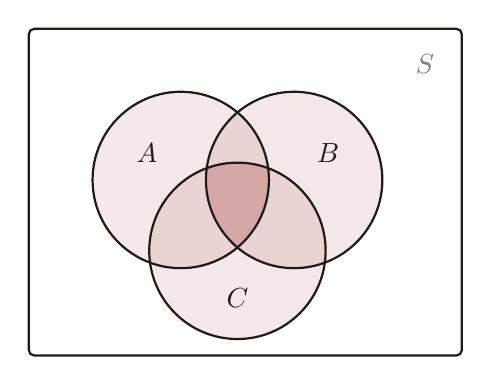
\begin{tikzpicture}[
  x=1cm,
  y=1cm,
  every node/.style={font=\normalsize}
]
  \draw[journalink, line width=0.8pt, rounded corners=2pt]
    (-2.65,-2.05) rectangle (2.85,2.1);

  \path[fill=journalaccent, fill opacity=0.11] (-0.72,0.18) circle (1.12);
  \path[fill=journalaccent, fill opacity=0.11] (0.72,0.18) circle (1.12);
  \path[fill=journalaccent, fill opacity=0.11] (0,-0.72) circle (1.12);
  \begin{scope}
    \clip (-0.72,0.18) circle (1.12);
    \clip (0.72,0.18) circle (1.12);
    \path[fill=journalaccent, fill opacity=0.18] (0,-0.72) circle (1.12);
  \end{scope}

  \draw[journalink, line width=0.8pt] (-0.72,0.18) circle (1.12);
  \draw[journalink, line width=0.8pt] (0.72,0.18) circle (1.12);
  \draw[journalink, line width=0.8pt] (0,-0.72) circle (1.12);

  \node[journalink] at (-1.15,0.52) {$A$};
  \node[journalink] at (1.15,0.52) {$B$};
  \node[journalink] at (0,-1.32) {$C$};
  \node[journalmuted] at (2.38,1.65) {$S$};
\end{tikzpicture}
\end{document}
